%\documentclass[../../talk.tex]{subfiles}
%\begin{document}


    	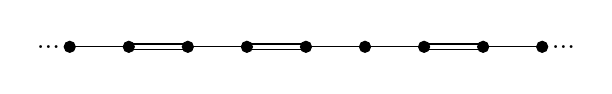
\begin{tikzpicture}[scale=.5]
    		\newcommand{\orig}{-1.5}
    		\newcommand{\trans}{1.5}
    		\newcommand{\vertspac}{-2.}
    		\newcommand{\vertsize}{0} % vertical span of the rectangles
    		\newcommand{\del}{.2}
    		\newcommand{\rad}{4pt} % radii of the circles

    		
    		% set the style of the strong bonds
    		\tikzset{
    			strong/.style={
    				double,
    				double distance=1.5\rad,
    				line width=0.5pt
    				}
    		}
    	
    		% initial chain
    	
    		% bonds 
        	\draw[-] (\orig, 0)  node [left] {...}  -- (\orig+\trans, 0) node [midway, below] {} node [midway, above] {\A};
			\draw[strong] (\orig+\trans,0) -- (\orig+2*\trans,0) node [midway, below] {}node [midway, above] {\B};
			\draw[-] (\orig+2*\trans,0) -- (\orig+3*\trans,0) node [midway, below] {}node [midway, above] {\A};
			\draw[strong] (\orig+3*\trans,0) -- (\orig+4*\trans,0) node [midway, below] {}node [midway, above] {\B};
			\draw[-] (\orig+4*\trans,0) -- (\orig+5*\trans,0) node [midway, below] {}node [midway, above] {\A};
			\draw[-] (\orig+5*\trans,0) -- (\orig+6*\trans,0) node [midway, below] {}node [midway, above] {\A};
			\draw[strong] (\orig+6*\trans,0) -- (\orig+7*\trans,0) node [midway, below] {}node [midway, above] {\B};
			\draw[-] (\orig+7*\trans,0) -- (\orig+8*\trans,0) node [right] {...} node [midway, below] {}node [midway, above] {\A};
    	
    		% sites
			\foreach \x in {0,...,8}
		      \filldraw (\orig+\x*\trans,0) circle (\rad); % node [below] {$\ket{\x}$};
		     
		    

		\end{tikzpicture}

%\end{document}